\documentclass[fleqn,10pt]{wlscirep}
\usepackage[utf8]{inputenc}
\usepackage[T1]{fontenc}
\usepackage{graphicx}
\usepackage{tablefootnote}
\usepackage{xr}

\makeatletter
\newcommand*{\addFileDependency}[1]{% argument=file name and extension
  \typeout{(#1)}
  \@addtofilelist{#1}
  \IfFileExists{#1}{}{\typeout{No file #1.}}
}
\makeatother


\newcommand*{\myexternaldocument}[1]{%
    \externaldocument{#1}%
    \addFileDependency{#1.tex}%
    \addFileDependency{#1.aux}%
}

\myexternaldocument{SI}

\title{NMRlipids Databank: Overlay Databank of Lipid Membrane Simulations Arising from Open Collaboration}

\author[1]{Anne Kiirikki}
\author[2]{...}
\author[1,*]{O. H. Samuli Ollila}
%\author[1,2,+]{Christine Author}
%\author[2,+]{Derek Author}
\affil[1]{University of Helsinki, Institute of Biotechonology, Helsinki, Finland}
\affil[2]{Affiliation, department, city, postcode, country}

\affil[*]{samuli.ollila@helsinki.fi}

%\affil[+]{these authors contributed equally to this work}

%\keywords{Keyword1, Keyword2, Keyword3}

\begin{abstract}
We present a databank of lipid bilayer simulations from the NMRlipids open collaboration project.
\end{abstract}
\begin{document}

\flushbottom
\maketitle
% * <john.hammersley@gmail.com> 2015-02-09T12:07:31.197Z:
%
%  Click the title above to edit the author information and abstract
%
\thispagestyle{empty}

%\noindent Please note: Abbreviations should be introduced at the first mention in the main text – no abbreviations lists. Suggested structure of main text (not enforced) is provided below.

\section{Introduction}

%The demand for sharing and reusing of MD simulation data is increasing, but practical solution remains unclear due to unsolved issues in data storage and indexing.

While MD simulations of systems with few biomolecules continue having major contributions in our understanding on biology and drug design, researches are now searching new avenues by building models not only for individual molecules but whole cells or organelles using interdisciplinary approaches~\cite{johnson15,thornburg22,gupta22}.

The importance of sharing MD simulation data following the FAIR principles~\cite{wilkinson16} has been widely recognized~\cite{feig99,tai04,silva06,abraham19,hildebrand19,hospital20,abriata20,espigares20}, and databanks are emerging~\cite{meyer10,kamp10,hospital16,mixcoha16,newport19,bekker20,espigares20,leston22}.
The relevance of quality evaluation of simulation trajectories in databanks regarding technical details of simulations and accuracy of the underlying physical description of the system (force field) has become evident~\cite{tai04,meyer10,hospital20} and such quality evaluation has in some cases also been implemented~\cite{meyer10,hospital16}. However, straightforward quality comparisons between individual simulations or force fields within these databanks remain challenging. 
While importance of such databanks for MD simulations is widely recognized~\cite{feig99,tai04,silva06,abraham19,hildebrand19,hospital20,abriata20,espigares20} and different kinds of approaches are emerging~\cite{meyer10,kamp10,hospital16,mixcoha16,newport19,bekker20,espigares20,leston22}, generally accepted protocols and best practices are still under active development.


Here we present a solution for lipid bilayers based on overlay databank structure illustrated in Fig.~\ref{fig:overlay}.  The concept of overlay databank is developed here to solve the practical challenges in generating databanks of MD simulation data enabling flexible analyses over large sets of simulation data, but it can be  potentially used for wide range of situations. Particularly when storage of raw data requires significant resources and final outcomes or best practices are not yet clear, overlay databank approach lowers the barrier to start without compromizing the long term stability or scalability.

The practical relevance of the NMRlipids databank is exemplified by automatic quality evaluation and ranking of large amount of MD simulation data, data-driven analysis detecting correlations between properties of model cell membranes and analyses of rare phenomena that are beyond the scope of standard MD simulation studies. The NMRlipids databank provides new tools for researchers in wide range of fields in academia and industry from cell membrane biology to lipid nanoparticle formulations and data-driven computational chemistry and machine learning. 

%The Introduction section, of referenced text\cite{Figueredo:2009dg} expands on the background of the work (some overlap with the Abstract is acceptable). The introduction should not include subheadings.

\section{Results}

%Up to three levels of \textbf{subheading} are permitted. Subheadings should not be numbered.
\subsection{Programmatic access to MD simulation data of membranes composed of most common biologically abundant lipids}
NMRlipids databank is a community driven databank containing atomistic MD simulations of biologically relevant lipid membranes emerging from the NMRlipids open collaboration~\cite{botan15,ollila16,catte16,antila19,bacle21}. Nearly thousand simulation trajectories with the total length approaching half a millisecond can be accessed programmatically using Python API or graphical user interface (\url{http://www.databank.nmrlipids.fi/}). NMRlipids databank is the only databank of MD simulations with open programmatic access to its content enabling fully flexible analyses of its content. Following the FAIR principles and NMRlipids project protocol, not only the content and computer programs related to the databank but also the whole construction process of the databank are open access~\cite{botan15}. The NMRlipids databank will be always open for data and other contributions.

The distribution of different lipid types in simulations in the NMRlipids databank (Fig.~\ref{fig:overlay}C) resembles the biological abundancies, the PC being the most common lipid type followed by PE, PS, PG, PI, and other lipids depending on organism and organelle~\cite{vanmeer08}. 
Currently the databank is composed of approximately 500 trajectories with the total length of approximately 231 microseconds of which most are contributed for the previous publications from the NMRlipids open collaboration~\cite{botan15,catte16,antila19,bacle21}. The distribution of lipids, force fields, length of the trjajectories and available binary mixtures are shown in Fig.~\ref{fig:overlay}. 


The three layer structure of the NMRlipids databank, illustrated in Fig.~\ref{fig:overlay} a, enables an efficient way to share and upcycle large MD simulation trajectories.  Layer 1 contains raw simulation data that can locate in any publicly available repository or server offering long term stability and permanent links to the data, such as digital object identifiers. Layer 2 contains all the relevant information on the simulations, including links to the raw data in layer 1 and relevant metadata describing the systems. Layer 3 is the application layer containing outputs from the databank, such as graphical user interface (\url{http://www.databank.nmrlipids.fi/}) and results from analyses desribed in sections below.   

Layer 2 is the core of the databank. In addition to the metadata and links to raw simulation data, it contains universal naming conventions for the molecules and atoms in the databank, computer programs to generate and analyse the databank, basic properties calculated from all simulations (area per lipid, C-H bond order parameters, x-ray scattering form factors and membrane thickness), and quality evaluation of simulations against experimental data. In practise, this information is stored is the git repository which is currently available at~\url{https://github.com/NMRLipids/Databank}.
Detailed description on its content is in the supplementary information. Applications in layer 3 uses the information in layer 2 to access raw data in layer 1 to perform automatic analyses over large sets of simulations in the databank. 

%are enabled by the 
%The databank can be used in layer 3 by accessing the raw data and information stored in the databank by employing the universal naming conventions for atoms, molecules and simulation details. The applications can be linked to the core databank (layer 2) without actually including them, thereby enabling flexible extension of the data without compromising the simplicity and lightness of the core databank.

\begin{figure}
    \centering
    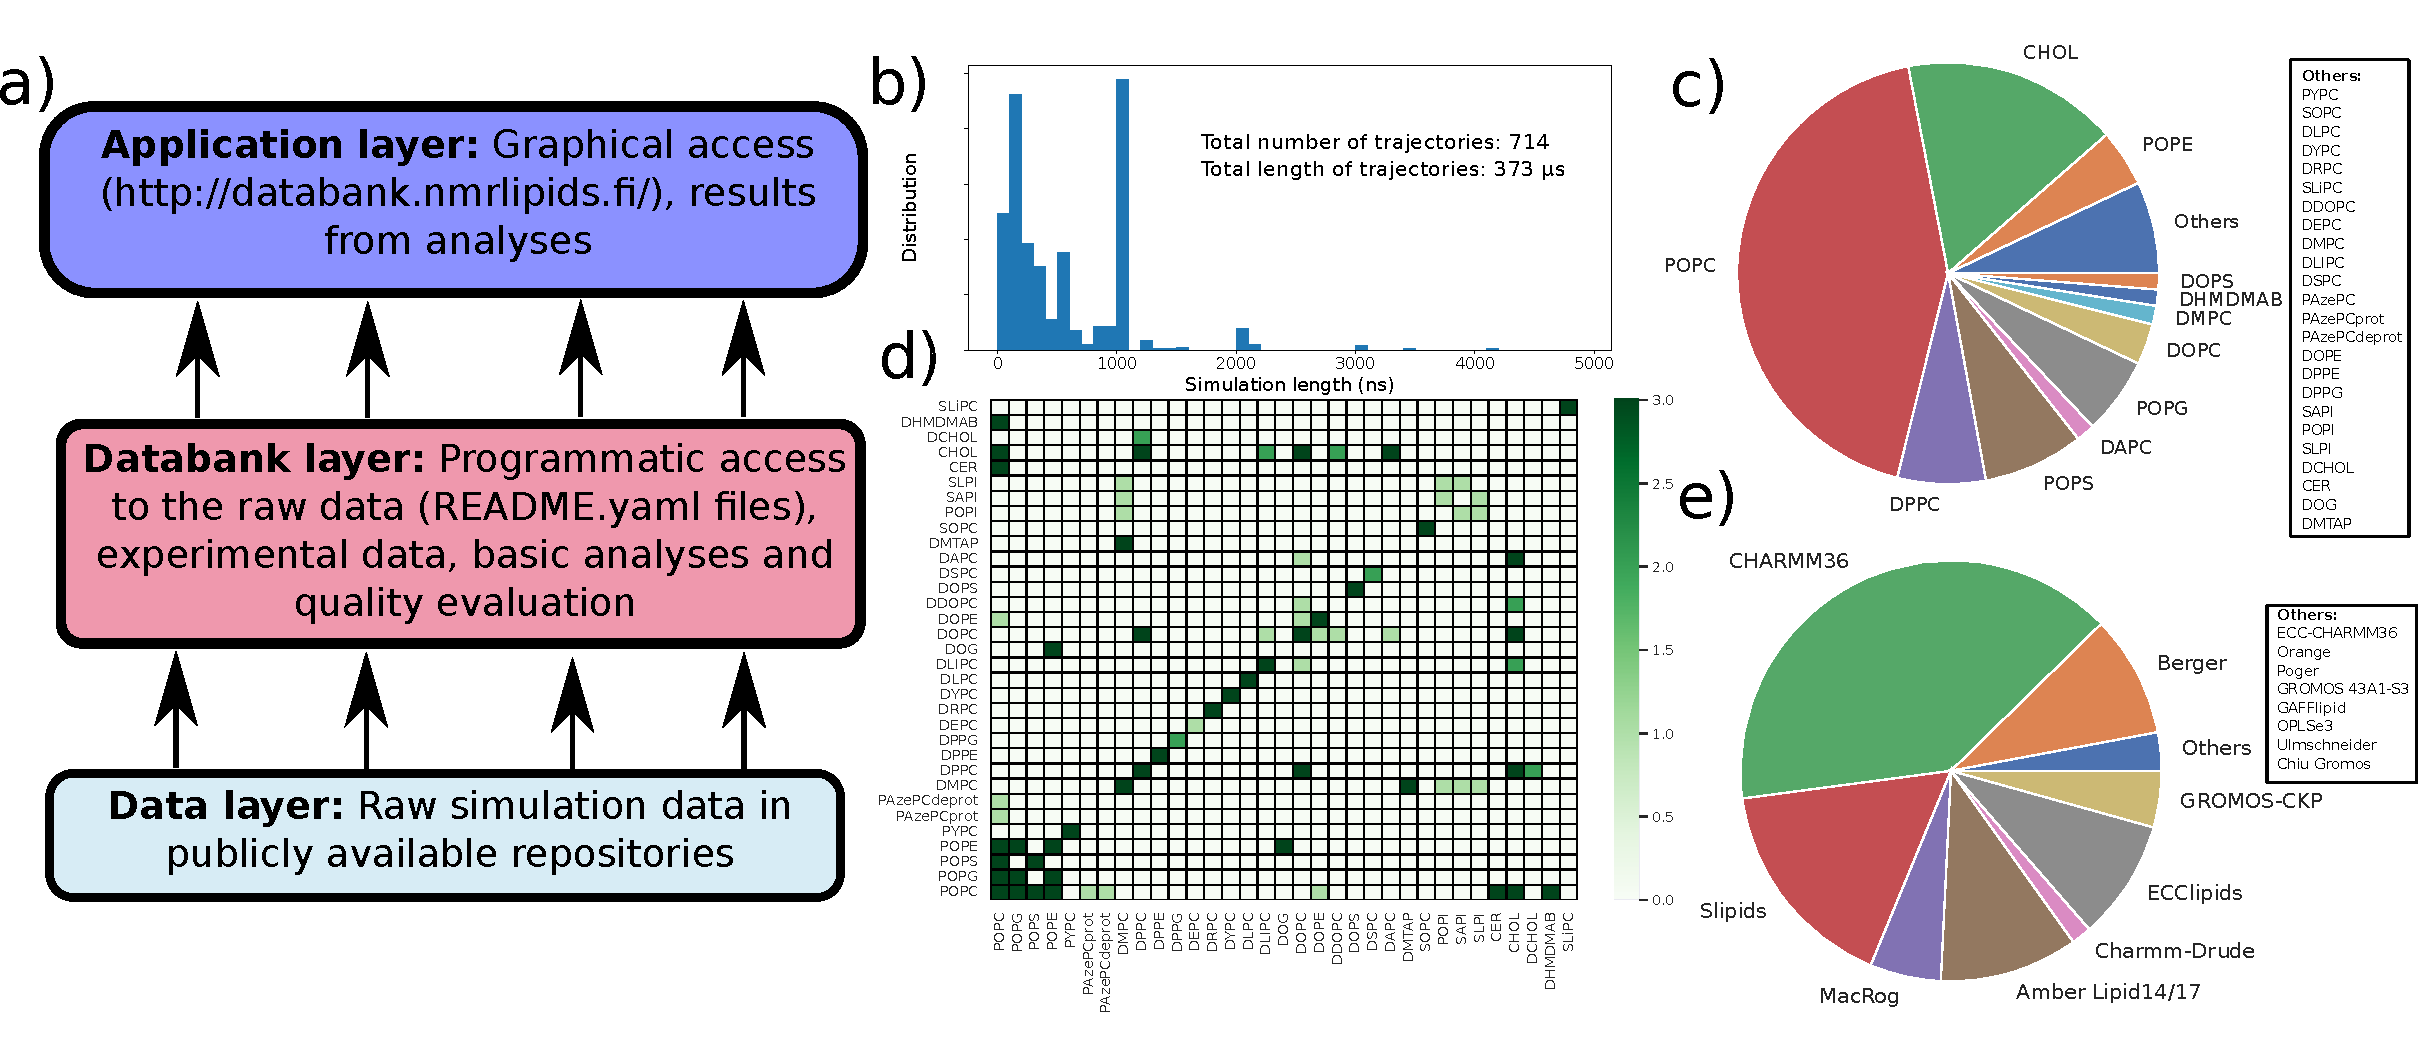
\includegraphics[width = 180mm]{Figures/overlay2.pdf}
    \caption{a) Structure of an overlay databank. 
    %Raw data is available from a publicly accessible repository (layer 1).
    %The core of the databank contains information on the location of the raw data and indexing of molecular %compositions and simulation details described with universal naming conventions (layer 2).
    %The content of databank can be viewed and analysed using external programs that automatically read the information and data from layers 1 and 2 (layer 3). Examples of such applications are the GitHub repository generating the results presented in this work and the graphical access to the databank.
    More detailed structure of the layer 2 in the NMRlipids databank is illustrated in Fig.~\ref{DatabankStructure} in the SI.
    b) Distribution of the lengths of the trajectories, total number of trajectories and total lenght of the simulations in the NMRlipids databank.
    c) Distribution of lipids present in the trajectories in the NMRlipids databank. Lipids occuring in five or less simulations ('others') are listed in the right. 
    d) Currently available binary mixtures in the NMRlipids databank. 
    e) Distribution of force fields in the simulations in the NMRlipids databank.
    The figures and numbers are created on 9th of May 2022.}
    \label{fig:overlay}
\end{figure}


\subsection{Quality evaluation of force fields}
Quality of membrane simulations with different force fields have been evaluated against experimental data during parameterization and in separate comparison studies~\cite{botan15,ollila16,catte16,pluhackova16,perez17,leonard19}, but universal quality measure for membrane simulations is not defined and controversial results are often reported from simulations~\cite{antila22b}. The lack of universal quality measure for membrane simulations complicates the selection of proper simulation parameters and the estimation of reliability in simulations, thereby being a major obstacle in many applications of membrane MD simulations. To enable the rapid quality evaluation of membrane MD simulations, a quantitative quality measure based on C-H bond order parameters from NMR experiments is defined in the NMRlipids databank. %Conformational ensembles of individual lipid molecules are evaluated against C-H bond order parameters from NMR experiments. 
This is complemented by comparing the locations of x-ray scattering form factor minima against experiments. 
%that are related to the overall membrane dimensions via electron density profile. 
Both of these are robust experimental measurables that can be directly connected to the simulation data~\cite{ollila16}. The used quality measures are defined in detail in the supplementary information.

%NMRlipids databank contains also experimental order parameter and x-ray form factor data that is connected to corresponding  simulations in order to define the simulation qualities and rank them to select the suitable simulation models for particular applications. 
Simulations with the highest scores based on order parameter evaluation for all simulations are shown in Fig.~\ref{fig:quality} A and for POPE lipids in Fig.~\ref{fig:quality} B. The direct comparison with experiments for the best simulation, POPC with OPLS3e, is shown in Fig.~\ref{fig:quality} C, where discrepancies with experiments are observed only for the third carbon in the $\it{sn}$-1 chain, and carbons 8 and 9 close to the double bond in $\it{sn}$-2 chain. The best overall quality for POPE is found in GROMOS-CKP simulation, for which the direct comparison in Fig.~\ref{fig:quality} D show minor differences in acyl chains, but major discrepancies in glycerol backbone and in the first carbon of $\it{sn}$-2 chain. These parts are better described for POPE by CHARMM36 parameters (direct comparison shown in Fig.~\ref{fig:quality} E), but its overall quality suffers from the overestimated order in acyl chains. 

\begin{figure}[tbp]
    \centering
    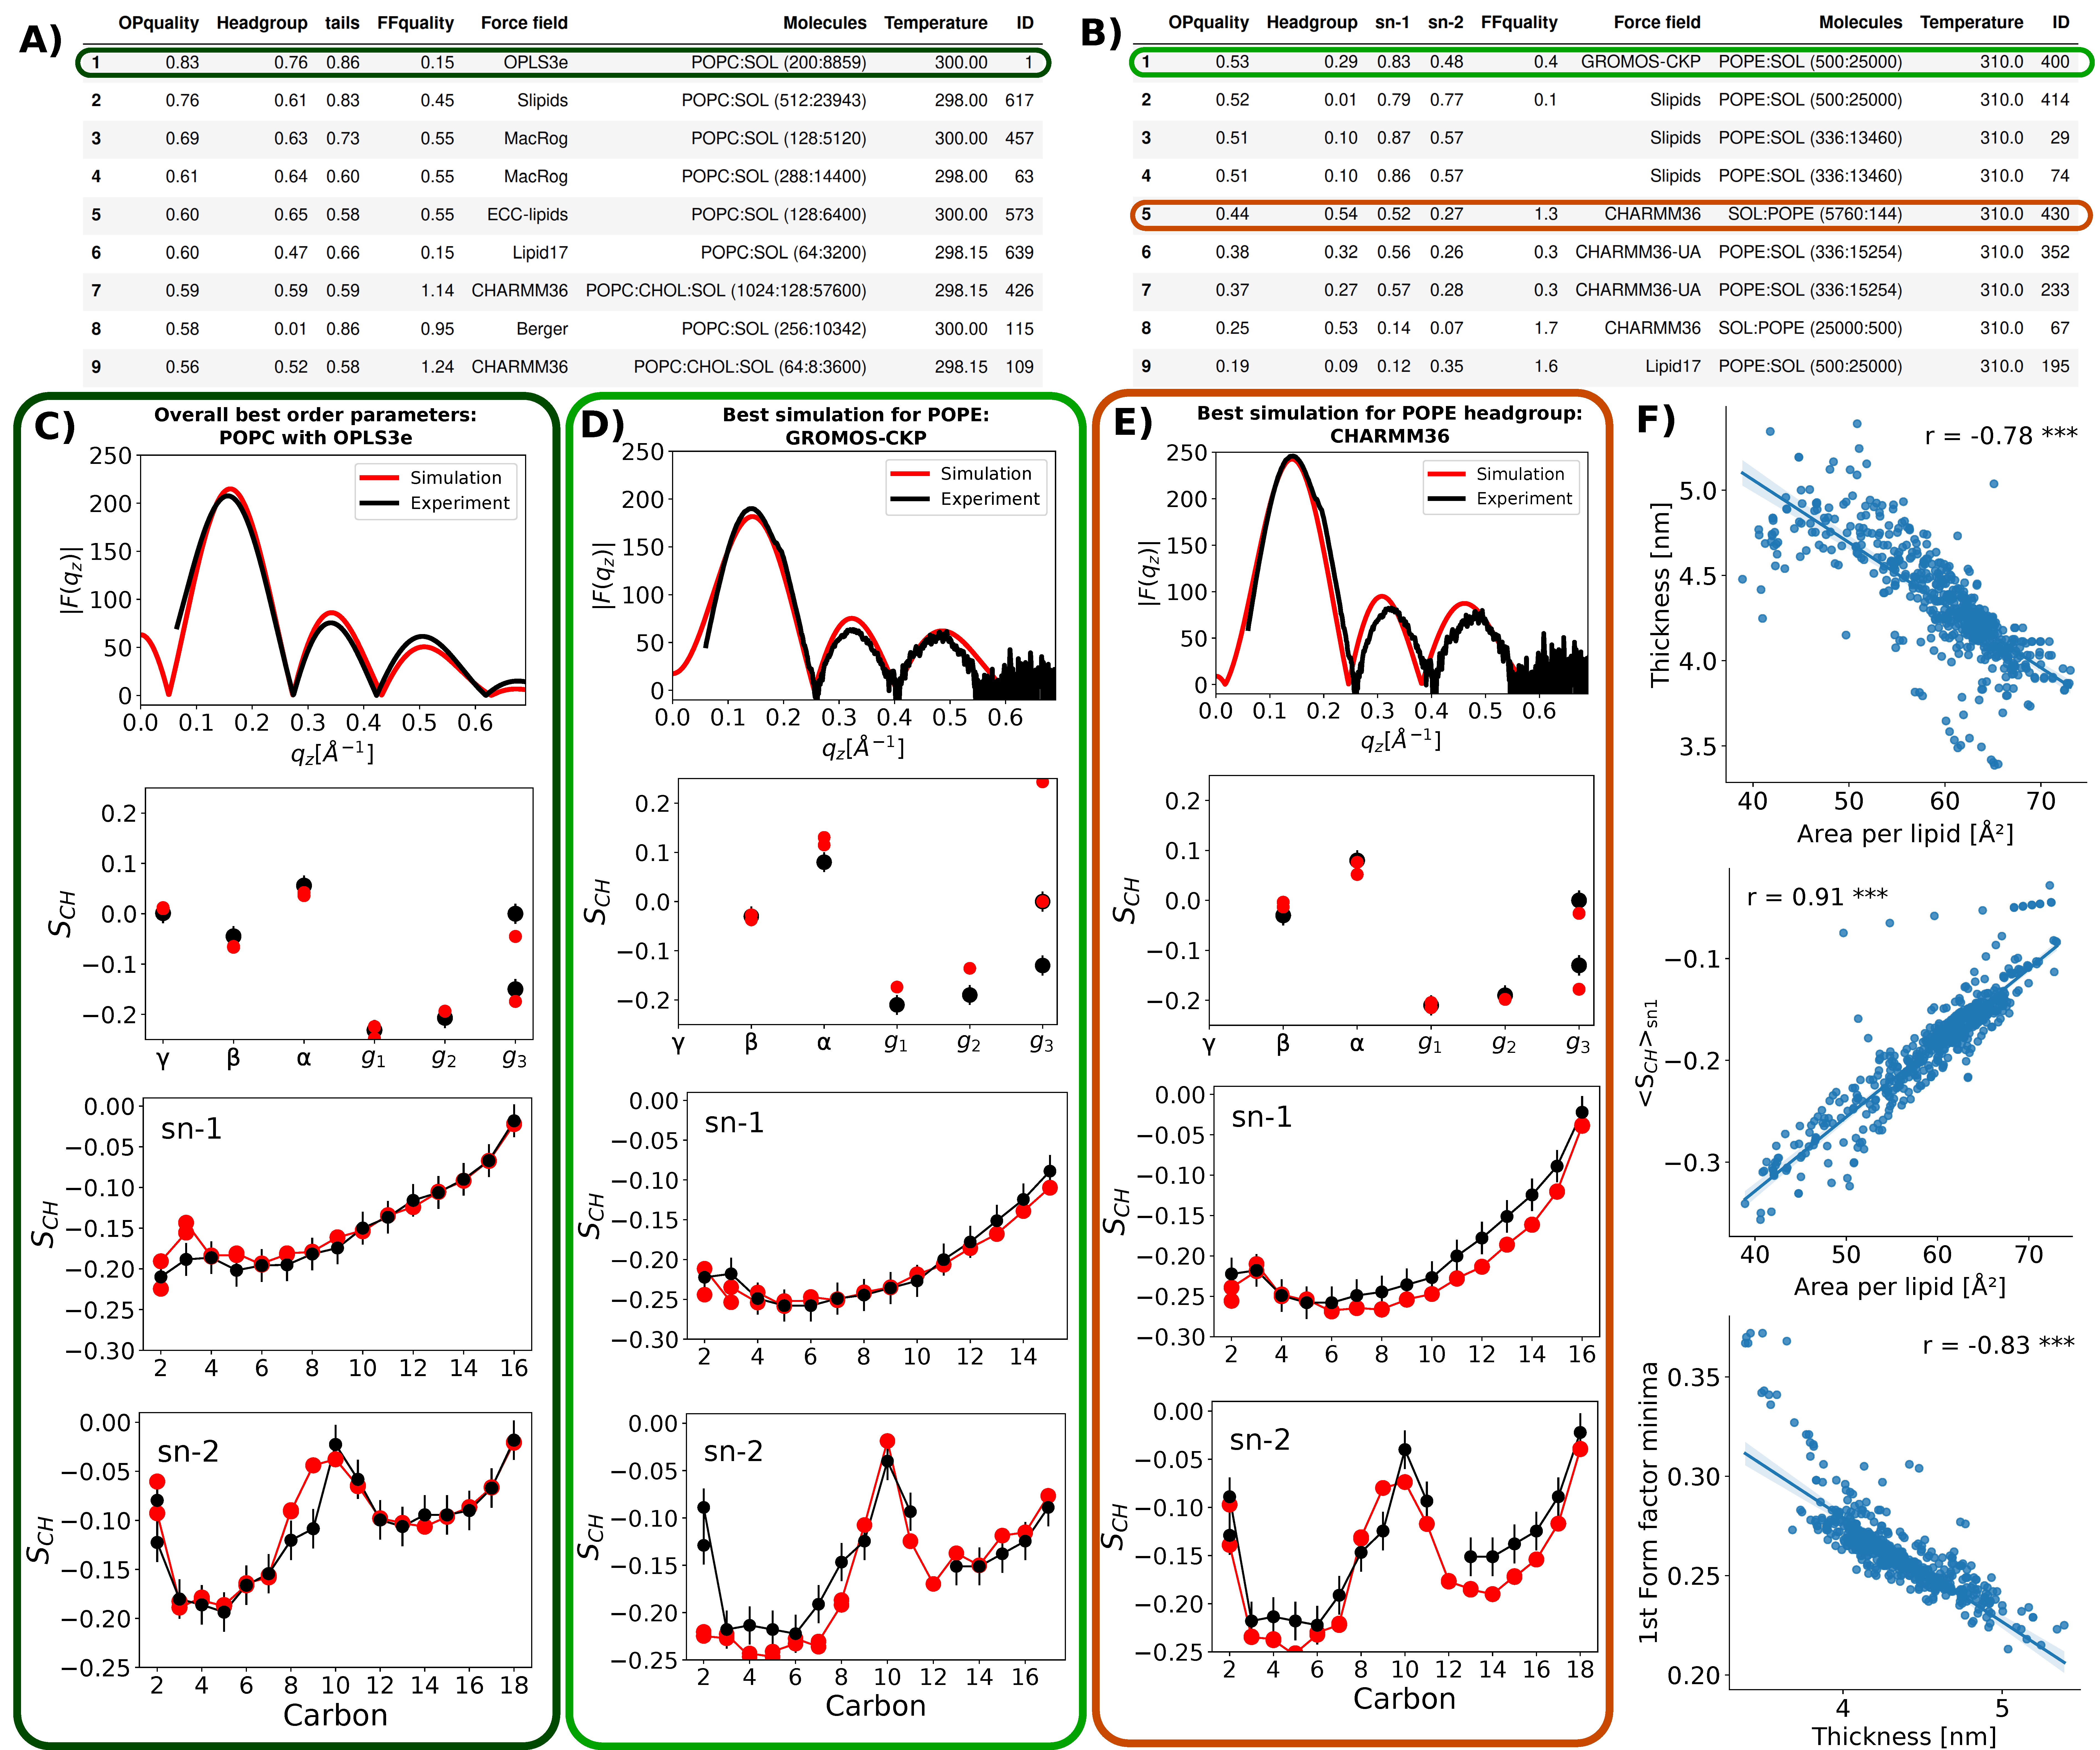
\includegraphics[width=180mm]{Figures/quality3.pdf}
    \caption{ A) Best simulations ranked based on overall order parameter quality.
    B) Best simulations ranked based on the overall order parameter quality of POPE lipid. 
    C) Scatter plots and Pearson correlation coefficients for the area per lipid, thickness, and experimental observables. 
    %second minima of form factor and average order parameter of the {\it sn}-1 acyl chain extracted from the NMRlipids databank. 
    All correlation coefficients have p-value below 0.001. For more correlations see Fig.~\ref{fig:QualityCorrelationsSI}.
    D)-F) Evaluation against experimental data exemplified for a simulation with the best overall order parameter quality (D), the best quality for POPE lipid (E), and the headgroup quality for POPE (F).
    %c) Change in area per lipid upon addition of POPE to POPC in different simulation extracted from the NMRlipids databank and quality evaluation table of POPE simulations.
    }
    \label{fig:quality}
\end{figure}

\subsection{Finding the best models for PC and PE lipid mixtures}
The power of the NMRlipids databank in finding the best models for a certain lipid bilayer system is exemplified here for mixtures of PE and PC lipids. Area per lipids from available POPC and POPE bilayer simulations in the databank from different force fields at 310\,K are shown in Fig.~\ref{fig:POPCPOPEapls}. Because the area per lipid strongly correlates with the average order of $\it{sn}$-1 chain (Fig.~\ref{fig:quality} F), we use order  parameter qualities to evaluate which simulations predict the best area per lipids for POPC and POPE. Among the force fields with area per lipids shown in Fig.~\ref{fig:POPCPOPEapls}, Slipids ranks 1st for POPC with a clear difference to others, and 2nd for POPE with only marginally lower quality than GROMOS-CKP (Figs.~\ref{fig:quality} A and B). The direct comparison with experiments in Fig.~\ref{fig:POPC_POPE_dataSI} in the supplementary information reveals that GROMOS-CKP and CHARMM36 predicts too ordered (too low area per lipid) bilayer for POPC, while the order parameters in Lipid17 are lower than in experiments indicating overestimated area per lipid. For POPE, order parameters in  Slipids and GROMOS-CKP are close to experiments suggesting that their are per lipids are most reasonable, while CHARMM36 and Lipid17 are too packed thereby overestimating the order parameters. 
\begin{figure}[tbp]
    \centering
    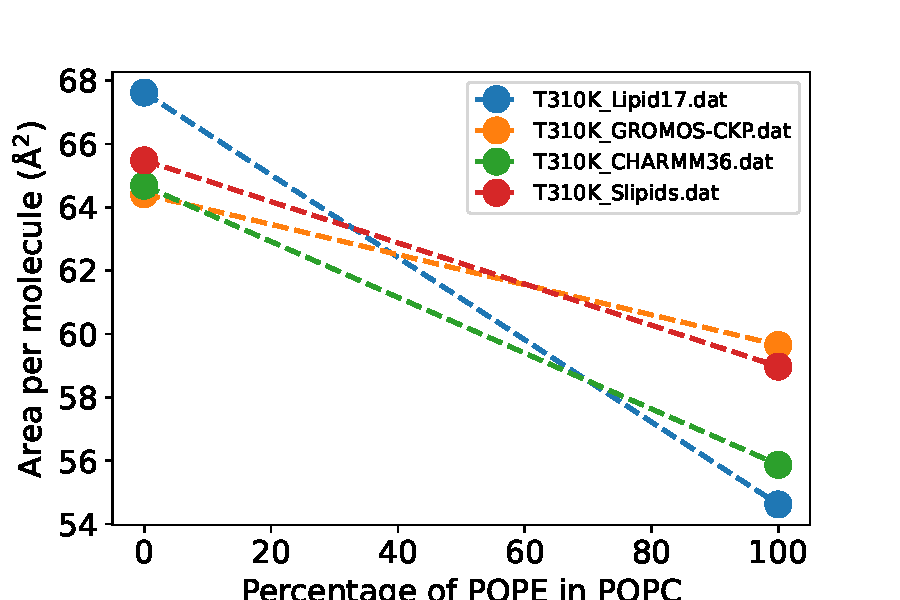
\includegraphics[width=88mm]{Figures/APL.pdf}
    \caption{Differences in area per lipids of POPC and POPE bilayers between different force fields.  
    }
    \label{fig:POPCPOPEapls}
\end{figure}


In conclusion, the quality evaluation based on the NMRlipids databank suggests that the Slipids parameters would give the most reliable description for membrane packing of POPC:POPE mixtures. Slipids was a relatively good model also for POPC:POPS mixtures in similar comparisons utilizing the preliminary version of the NMRlipids databank~\cite{antila22b}, although charged membranes are more complicated as the counterion binding affinity plays a significant role in membrane packing~\cite{antila19}. On the other hand, CHARMM36 overcomes Slipids when the focus is on conformational ensembles of headgroups  in different types of lipids because the accuracy of glycerol backbone is low in Slipids~\cite{bacle21}. Altogether, these examples demonstrate how the NMRlipids databank can be used to navigate in the complex landscape of lipid force field quality.


%On the other hand, the first form factor minima is correlated stronger with membrane thickness (Fig.~\ref{fig:quality} C) than with the area per lipid (Fig.~\ref{fig:QualityCorrelationsSI}). 
%Scatter plots and Pearson correlation coefficients in Fig.~\ref{fig:quality} C reveal strong correlation between membrane area per lipid and thickness.


%Understanding such complex picture of lipid bilayer MD simulation quality would not be possible without automatic quality evaluation of large sets of simulations enabled by the NMRlipids databank.

%The power of NMRlipids quality metrics in selecting the best model for particular application is demontrated in Fig.~\ref{fig:quality} c) where the area per lipids of POPC:POPE mixtures from different force fields are shown and quality of POPE simulation in different force fields are evaluated. 



 %This is demonstrated in Fig.~\ref{fig:quality} a) showing correlations between membrane lateral density (area per lipid), thickness, minima of form factor and acyl chain order analyzed from all apporimately 500 trajectories in the NMRlipids databank. Membrane area per lipid has negative correlations with membrane order and thickness with Pearson coefficient of -0.78 and -0.49, respectively, because decreased area leads to more ordered, tightly packed and stretched acyl chains leading to thicker membranes. On the other hand, locations of form factor minima have positive correlation with the membrane area and negative correlation with the thickness. In conclusion, both x-ray scattering form factors and acyl chain order parameters from NMR are on average good proxies for membrane packing and thickness, while NMR order parameters give segmental resolution information on the quality of conformational ensembles of lipids.




\subsection{Water diffusion anisotropy in membrane systems}
The anisotropy in water diffusion in parallel and perpendicular directions with respect to membranes plays a role in the drug translocation through biological material, particularly in skin \cite{hansen13,wen18,nitsche19,roberts21}, and in MRI imaging~\cite{topgaard20}. Several models on how water dynamics depends on membrane properties have been proposed based on different experimental and theoretical methods, yet consensus 
%on how water permeability depends on membrane properties, such as area per lipid and thickness, or molecular composition, 
has not been reached~\cite{mathai07,nitsche13,nitsche16,shinoda16,venable19,frallicciardi22}. MD simulations have been also used in these endeavours, but systematic studies are limited by the accessible amount of data as only few water permeation events are typically observed in a single MD simulation trajectory~\cite{venable19,camilo2022}. Therefore, this serves as an excellent example where the large amount of available MD simulations in the NMRlipids databank can be utilized to answer important biological questions.

To this end, we first calculated the water permeability through membranes from all the simulations in the NMRlipids databank. Resulting permeabilities are shown as a function of temperature, membrane thickness, area per lipid, and acyl chain order in Figs.~\ref{fig:permeability} B-E. The values for water permeabilities from simulations vary between 0.3 and 322\,$\mu$m/s with the mean and median of 14\,$\mu$m/s and 8\,$\mu$m/s, respectively. These values have the same order of magnitude as the experimentally determined diffusive permeability coefficients, but are on average below the values reported for PC lipids in liquid crystalline phase,~190-330\,$\mu$m/s~\cite{jansen95}. To analyze how water permeability through membranes depend on bilayer properties on average, we calculated the average permeabilities over all systems with the value of temperature, thickness, area per lipid, or acyl chain order within a fixed range. These averaged permeabilities also shown in Figs.~\ref{fig:permeability} with black dots. As expected, the permeability increases with the temperature, giving 17\,$\pm$\,4\,k$_b$T for the average energy barrier for the water permeation from the Arrhenius plot in Fig.~\ref{fig:permeability} B. Water permeability decreases with increasing membrane packing, i.e., with decreasing area per lipid and increasing thickness and acyl chain order. Linear dependence of permeability on area per lipid and thickness is previously reported from simulations and experiments for some systems, but not for all~\cite{mathai07,venable19,frallicciardi22}. Our results suggest on average linear dependence for thicknesses above $\sim$\,3.9\,nm and area per lipids below $\sim$69\,Å$^2$ (insets in Figs.~\ref{fig:permeability} C-D), yet stronger dependence is observed for more loosely packed membranes. 
%within the range of experimentally reported values  permeability which is 1-2 orders of magnitude slower than osmotic permeability \cite{jansen95,??}. 
Clear dependencies of permeability on charged lipids, cholesterol, POPE, or hydration level were not observed in Fig.~\ref{fig:permeationSI} in the supplementary information.
%, although weak decrease for the latter two may be visible.

\begin{figure}[tb]
    \centering
    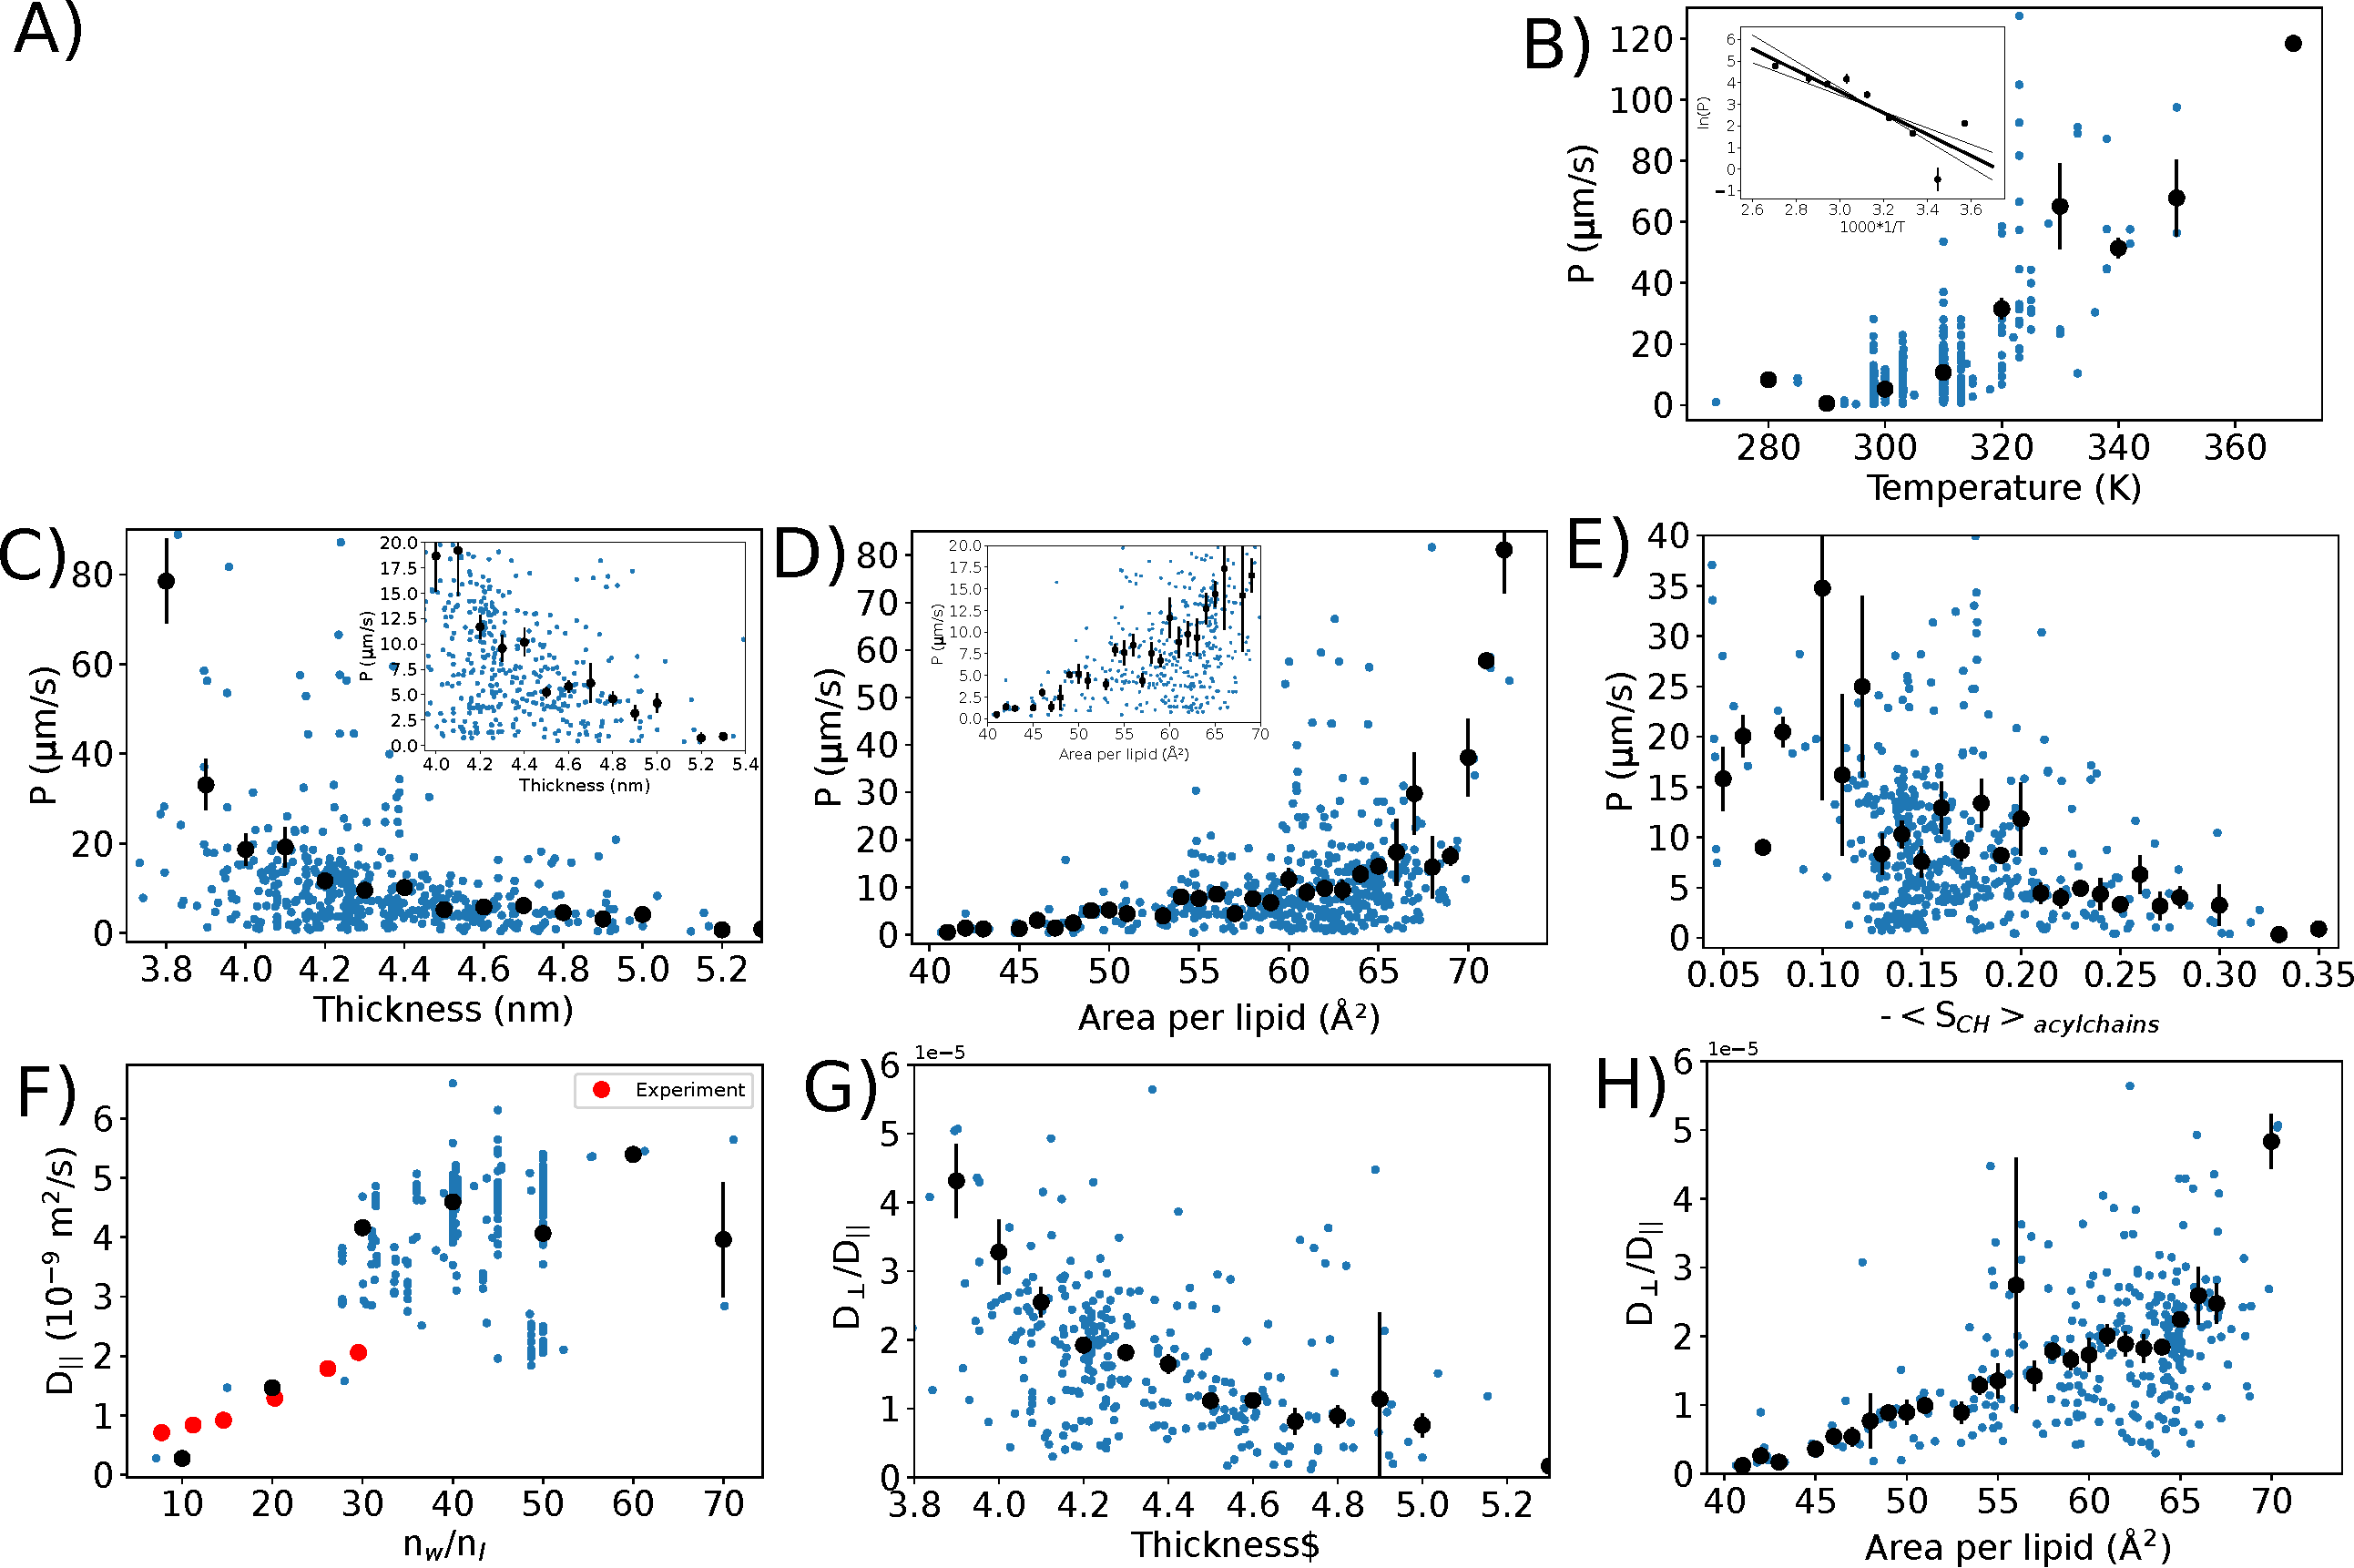
\includegraphics[width=180mm]{Figures/permeation2.pdf}
    \caption{{\bf A} Water diffusion, $D_\perp$, and permeability, $P$, through membranes, and lateral diffusion along the membrane, $D_{||}$, illustrated in a multilamellar stack of lipid bilayers. 
    {\bf B-E} Water permeation through membranes analyzed from the databank as a function of temperature, thickness, area per lipid, and acyl chain order. Values from simulations with non-zero permeation values are shown with blue dots. Averages over fixed range of x-axis values are shown with black dots. Insert in B) shows the Arrhenius plot of permeation ($\ln$ (P) vs. 1/T) that gives 17\,$\pm$\,4\,k$_b$T for the average activation energy for water permeation through lipid bilayer. Inserts in C) and D) show the region where the dependence could be considered approximately linear.
    {\bf F} Lateral diffusion of water as a function of hydration level. Experimental points for DMPC bilayers at 313\,K at different hydration levels are shown~\cite{rudakova04}.
    {\bf G-H} Diffusion anistoropy of water as a function of thickness and area per lipid. }
    \label{fig:permeability}
\end{figure}

To analyze the anisotropic diffusion of water in membrane environment, we also calculated the water diffusion parallel to the membrane surface from all simulations in the NMRlipids databank. The results at different hydration levels are shown in Fig.~\ref{fig:permeability} F together with the experimental data~\cite{rudakova04}. 
%The experimental water diffusion increases with increasing hydration level toward the value for bulk water . 
%As expected, water translational diffusion increase in the diffusion is observed with the increased temperature and hydration level (Figs.~\ref{fig:permeability} H and~\ref{fig:diffusionSI} B). 
Simulation results are close to the experimental values with low hydration levels, but increase to the values of approximately two times higher than experimental bulk water diffusion value (3.1$\cdot$\,10$^{-9}$\,m$^2$/s at 313\,K~\cite{khakimov08}) with high hydration levels. This is not surprising as the most common water model used in membrane simulations, TIP3P, overestimates the bulk water diffusion~\cite{pathirannahalage21}. The water diffusion parallel to membrane surface increased with the temperature, but dependencies on membrane area per lipid, thickness, or fraction of charged lipids were not observed in Fig.~\ref{fig:diffusionSI} in the supplementary information. In order to estimate the diffusion anistoropy of water in multilamellar membrane system, we translated the water permeation coefficients through membranes to diffusion coefficients through multilamellar stack using the Tanner equation~\cite{tanner78,wasterby02}. The resulting diffusion coefficients through the membranes are approximately five orders of magnitude slower than along the membrane (Figs.~\ref{fig:permeability} G and H), which is at the upper limits of the anisotropic estimated from the experimental data~\cite{nitsche19}. Relatively high anisotropy is understandable as simulations give slightly slower permeation rates and higher lateral diffusion rates than experiments. Significant increase in the diffusion anisotropy with membrane packing is observed, as $D_{\perp}/D_{||}$ drifts away from one with decreasing area per lipid and increasing thickness in Figs.~\ref{fig:permeability} G and H. This follows from decreasing water permeability with membrane packing (Figs \ref{fig:permeability} C and D), while lateral diffusion remains approximately constant (Fig. \ref{fig:diffusionSI} A and C). 

\subsection{Flip-flops}
Lipid flip-flops from one bilayer leaflet to another play an important role in lipid trafficking and regulating membrane properties~\cite{vanmeer08}. Phospholipid flip-flops are slow, occuring with the timescales of hours or days, while cholesterol, diacylglycerol and ceramide flip-flops are faster, yet the reported timescales range between minutes to sub-millisecods~\cite{vanmeer08,steck12,parisio16,gu19}. Flip-flops have been previously studied mainly with coarse-grained simulations and free energy calculations due to time scale limitations in atomistic simulations~\cite{parisio16}, but direct analyses on cholesterol flip-flops in atomistic simulations have been also emerging in recent years~\cite{gu19,javanainen18,baral20}. However, systematic studies on how flip-flop rates depend on membrane properties are still challenging even with the state of the art computational resources. The NMRlipids databank can greatly advance such studies by giving an easy access to large amounts of data simultaneously.

\begin{figure}[htb]
    \centering
    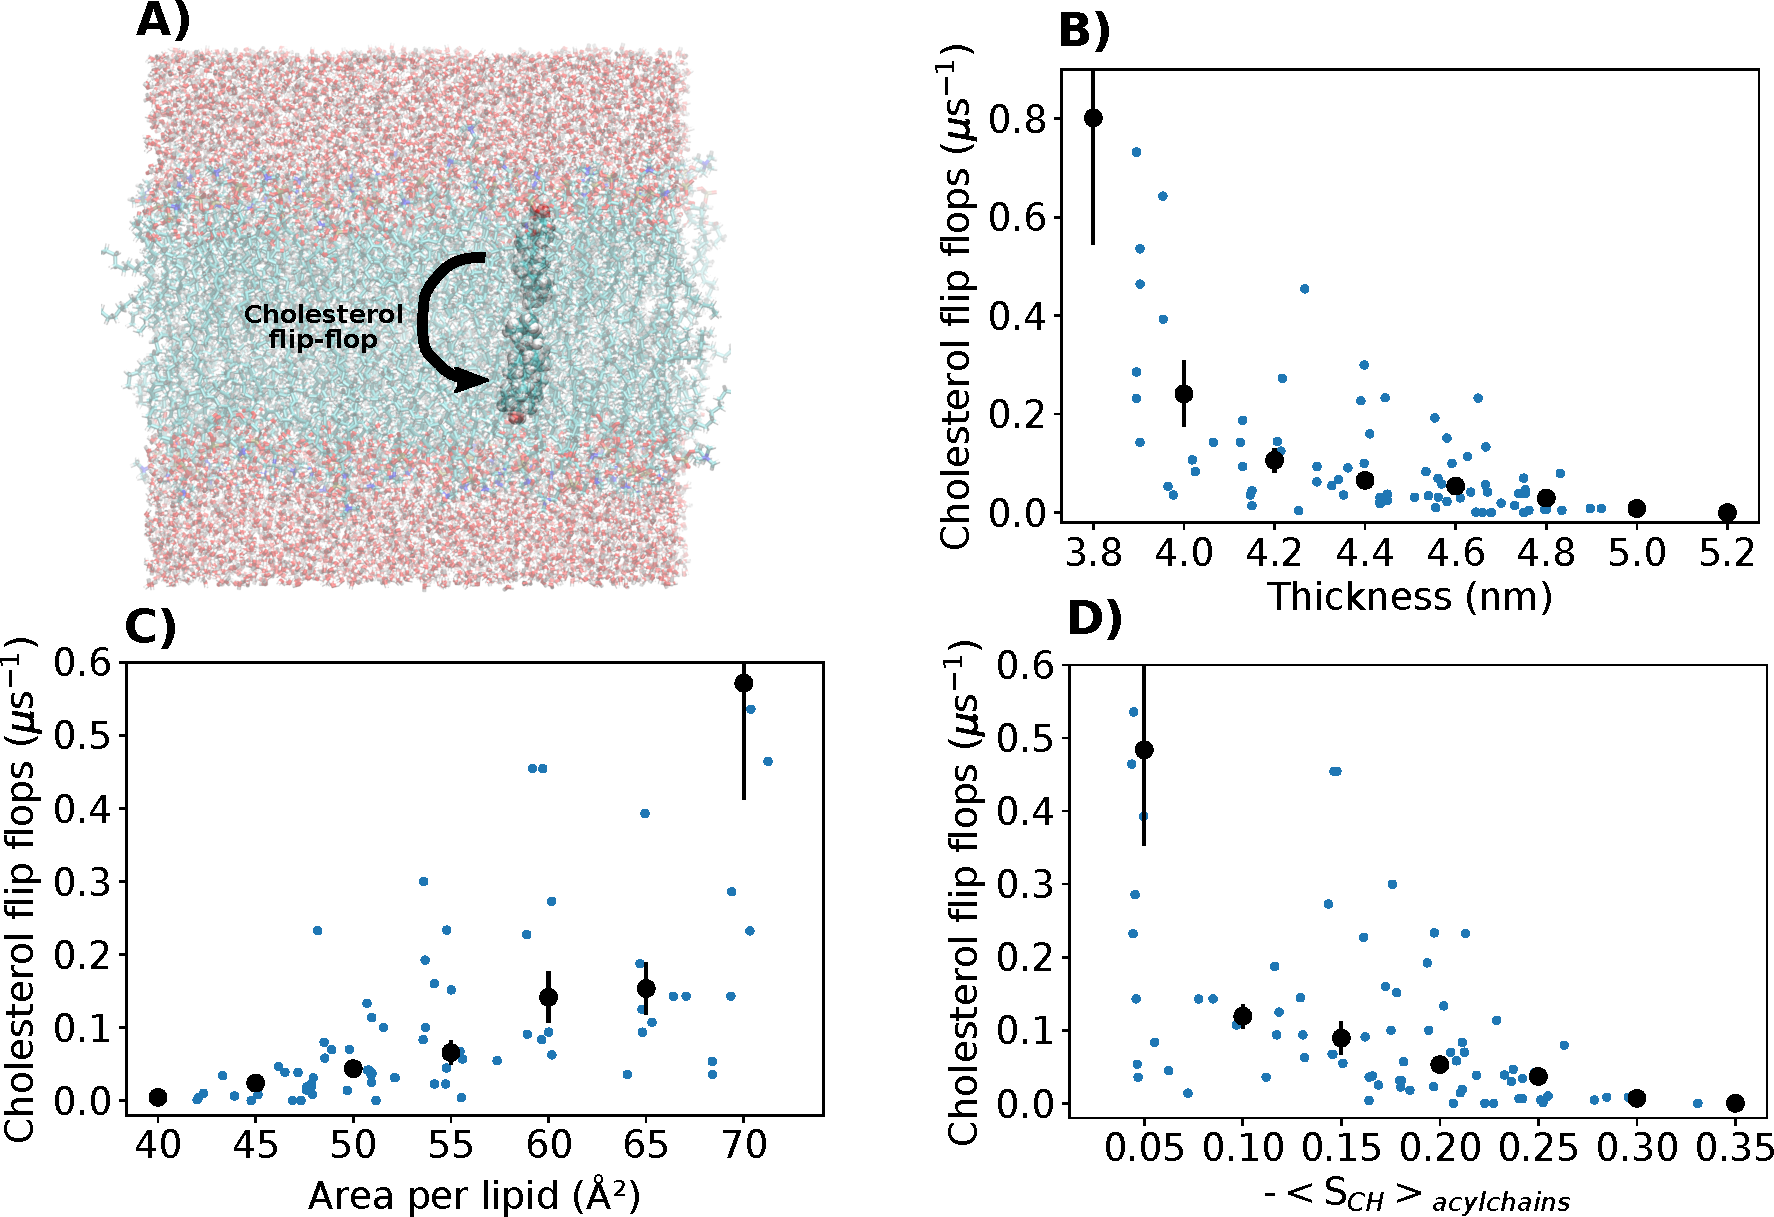
\includegraphics[width=88mm]{Figures/CholFlipFlops.pdf}
    \caption{{\bf A} Illustration of cholesterol flip-flop.  
      {\bf B-D} Cholesterol flip-flops analyzed from the databank as a function of membrane thickness, area per lipid, and acyl chain order.
      Values from simulations with non-zero flip-flop rates are shown with blue dots. Averages over fixed range of x-axis values are shown with black dots.
    }
    \label{fig:permeability}
\end{figure}



\section{Discussion}

%The Discussion should be succinct and must not contain subheadings.

Applications of MD simulations in understanding biomolecular behaviour are steadily increasing, but protocols for quality evaluation and sharing simulation data fall behind the ones in more elaborated fields, such as structural biology. Development of such protocols has been limited by practical challenges, such as lack of universally defined quality measures for MD simulations, incompatible naming conventions in different models and simulation softwares, and high technical requirements for hardware to share large trajectories from MD simulations, as well as incentives for scientist to evaluate and share their MD simulation data. 

The NMRlipids databank circumvents these challenges by utilizing the overlay databank design and open collaboration approach developed in the NMRlipids project~\cite{botan15}. In the overlay databank, the storage of large simulation files is outsourced to existing publicly available repositories while databank itself is essentially a git repository with open access licence containing relevant information about the trajectories, including the location of the raw data. This architecture streamlines the construction and maintenance of the databank
%Building accessible databanks of molecular dynamics simulation data has been challenging due to the required long term support for hardware and software maintenance. 
%
%, the demand of hardware can be distributed and open collaboration model reduces the risk for ending software maintenance. 
%Furthermore, the 
by distributing the long term commitment for hardware and software maintenance. Incentive to share the data is created in the NMRlipids open collaboration by offering authorship in published articles to the contributors.
%, thereby creating an incentive for contributions. 
Universal quality measures and naming conventions for molecules and atoms are defined in the NMRlipids databank to enable the automatic quality evaluation and other analyses.
%of lipid bilayer MD simulations introduced in the NMRlipids databank enables rapid ranking of available simulation models agains experimental NMR and x-ray scattering data. 
%
The current NMRlipids databank contains only lipid bilayer simulations, but the concept combining open collaboration and overlay databank structure can be applied also in other fields where similar barriers to establish publicly accessible databanks exist. 
%
%, thereby not requiring large resources to handle and maintain. 
%This lowers the barrier for starting such databank as well as for long term storage. 
%The NMRlipids databank  
%In addition to all computers where the databank is developed and used, the NMRlipids databank git is stored to Zenodo server, thereby enabling a very cost effective long term storage for the databank. 

The NMRlipids databank will be of great benefit to scientists involved in MD simulations. They will be able to rapidly evaluate the quality of MD simulations in order to filter out potentially misleading results or facilitate force field parameter development~\cite{antila22b}. The selection of best models for a specific application is demonstrated for PC/PE lipid mixtures in Fig.~\ref{fig:quality}, and previously for PC/PS lipid mixtures~\cite{antila22b}, and lipid headgroups~\cite{bacle21}. On the other hand, programmatic access in the NMRlipids databank enables automatic analyses over large sets of simulation data containing more data in terms of quantity (e.g., simulation length and number of conformations) with broader range in terms of content (e.g, lipid compositions and ion concentrations) that can be accessible for a single research group. Added value of the access to broad range of systems is exemplified in Figs.~\ref{fig:quality}~and~\ref{fig:permeability} revealing correlations between membrane properties, while large quantity of data enables the detection of rare phenomena with good statistics, as exemplified for water permeability in Fig.~\ref{fig:permeability} and cholesterol flip-flop events in Fig.~\ref{??}. 

Providing programmatic access to large scale MD simulation data can lead to applications in unprecedented directions. For example, water anisotropic diffusion analyzed in Fig.~\ref{fig:permeability} is relevant not only in pharmacokinetics but also in the development of MRI imaging methods where MD simulations are not yet widely used~\cite{topgaard20}. We expect the access provided by the NMRlipids databank to facilitate novel applications also in other fields where MD simulations are less commonly applied, such as design of lipid nanoparticles for drug delivery or other applications, and material science. The increasing amount of data in terms of quantity and content will also increase the scope of potential applications of the NMRlipids databank in time.

The NMRlipids databank can also serve as a training set for diverse machine learning applications. Most straightforward applications include models that would predict connections between membrane properties that are already stored in the databank. For example, a machine learning model predicting electron density profiles from form factors would be highly useful in interpretation of scattering experiments. On the other hand, more elaborated models could be trained to predict arbitrary membrane properties using the data from the NMRlipids databank. Such models could be used to connect membrane composition to relevant membrane properties in wide range of fields from molecular biology to drug development and biomolecular imaging. The overlay databank design can open such avenues also for other biomolecules than lipids, such as disordered proteins and membrane-protein systems.

Different types of applications enabled by the NMRlipids databank in wide range of fields are exemplified in Table~\ref{tab:applications}. 

\begin{table}[]
    \centering
    \begin{tabular}{p{5.0cm}  p{5.0cm}  p{4.0cm}}
    Type of application     & Practical examples & Target group \\
    \hline
    Analyses of rare phenomena               & Lipid flip-flops, water permeation & Membrane scientists \\
    \\
    Correlations between membrane properties & 
    Membrane structural properties, water dynamics (Figs.~\ref{fig:quality} and~\ref{fig:permeability}) & 
    Membrane scientists \\
    \\
    Applications that are outside typical scope of MD simulations & 
    Anisotropic water diffusion for pharmagokinetics and MRI imaging applications & 
    Scientist in fields where MD simulations are not usually applied \\
    \\
    Selection of the best simulation model for a specific application & 
    Best model for POPC lipids (Fig.~\ref{fig:quality}), headgroup conformations~\cite{bacle21}, 
    packing of PS~\cite{antila22b} and PE (Fig.~\ref{fig:POPCPOPEapls}) containing membranes. &
    Scientists using MD simulations \\
    \\
    Guidance for force field development & 
    Improvements in ion binding to lipids~\cite{melcr18,melcr20} and lipid headgroup conformational ensembles~\cite{??} &
    Scientists developing parameters for MD simulations \\
    \\
    Training and target data for coarse grained models & 
    Optimizing parameters of coarse grained models against NMRlipids databank, extracting continuum parameters for membranes. &
    Scientists developing and using coarse grained MD simulations \\
    \\
    Training set for machine learning applicatons &
    programmatic access to the data and results enables training of machine learning type of models for various applications, such as predictions of membrane properties from composition & Scientists building and using machine learning applications for biomolecules.  
    \end{tabular}
    \caption{Examples on applications of the NMRlipids databank.}
    \label{tab:applications}
\end{table}


\section{Methods}

%Topical subheadings are allowed. Authors must ensure that their Methods section includes adequate experimental and characterization data necessary for others in the field to reproduce their work.

\subsection{Structure of the databank}
Structure of the NMRlipids databank is illustrated more detailed in Fig.~\ref{DatabankStructure} in the supplementary information. The databank locates as a git repository at \url{https://github.com/NMRLipids/Databank/} and is permanently stored in Zenodo repository (\url{www.zenodo.org})~\cite{??}. Whenever a specific file is referred here, the file path within the NMRlipids databank repository is given. The scripts in the NMRlipids databank are mainly written in Python and many of them utilize the MDAnalysis module~\cite{gowers2019mdanalysis,michaud2011mdanalysis}.

The core content of the NMRlipids databank is stored in README.yaml files located at {\it /Data/Simulations} in the NMRlipids databank repository. Essential information for each simulation entry in the databank is stored in these files. These yaml files are both human and machine readable, and contain access to all information that are needed for further analyses of the simulations. The keys available in these files and their explanations are listed in table~\ref{tab:READMEkeys} in the supplementary information. To keep the databank light, the raw MD simulation data is stored in an external location which can be any stable publicly available repository, although all the current data locates in Zenodo \url{www.zenodo.org}. Whenever needed, the raw data can be downloaded through the links stored in the README.yaml files.  



\subsection{Molecule and atom naming convention} \label{naming}
Molecule and atom names used in a simulation are often needed when analyzing the simulation trajectories. However, the naming conventions of lipid molecules and atoms therein vary between authors and force fields because universal naming convention has not been defined. Because such convention is necessary for automatic analyses over simulations, we have defined the unique naming conventions for lipid molecules and atoms in the NMRlipids databank. For each molecule we have defined an unique abbreviation which are listed in table~\ref{tab:abbreviations} in the supplementary information. On the other hand, unique names for each atom in a molecule are defined and connected to corresponding names in a simulation using mapping files. Mapping files are in yaml format where unique atom names are connected to force field specific names. Also residue names and fractions lipids (headgroup, glycerol bakcbone, and acyl chains) can be defined in the mapping file. For example, the mapping files used in the NMRlipids databank are located at {\it /Scripts/BuildDatabank/mapping\_files} in the NMRlipids repository. For more details about mapping files, see~\url{https://nmrlipids.blogspot.com/2022/04/new-yaml-format-of-mapping-files.html}). In practise, information about molecule and atom names are given in the COMPOSITION dictionary in README.yaml files, where force field specific molecule name corresponding the unique abbreviation (table~\ref{tab:abbreviations}) and the name of the mapping file are given. 

%Upon addition of a new entry in the databank, the molecule names in the simulation corresponding the unique names and mapping files (available at \url{https://github.com/NMRLipids/Databank/tree/main/Scripts/BuildDatabank/mapping_files}) are defined in the dictionary. 

\subsection{Adding data into the NMRlipids databank}
In order to add a simulation entry into the NMRlipids databank, an initial info.yaml file containing user given information listed in table~\ref{tab:READMEkeys} needs to be created. For examples of these files, see {\it /Scripts/BuildDatabank/info\_files} in the NMRlipids databank repository. Using this file as an input, the {\it /Scripts/BuildDatabank/AddData.py} script then calculates the rest of the information to be stored in the README.yaml files, also listed in table~\ref{tab:READMEkeys}. The databank is open for submission of these info.yaml files via pull requests to the git repository. Large fraction of the current content is composed of the data uploaded to Zenodo in previous NMRlipids projects~\cite{botan15,catte16,antila19,bacle21}, yet also other simulation data from the Zenodo repository are added.

\subsection{Experimental data}
Experimental data used in the quality evaluation, currently composed of C-H bond order parameters and x-ray scattering form factors, are stored in {\it /Data/experiments} in the NMRlipids databank repository. Similarly to simulations, each experimental data set has a README.yaml file containing all the relevant information about the experiment. The keys and their descriptions for the experimental data are given in table~\ref{tab:READMEkeysEXP}. NMR data currently in the NMRlipids databank are taken from Refs.~\citenum{??} and x-ray scattering data from Refs.~\citenum{??}. In addition, some previously unpublished NMR and x-ray scattering data are used. These are measured with previously established methods as described in the supplementary information. 

\subsection{Calculation of C-H bond order parameters}
The C--H bond order parameters were calculated directly from the carbon and hydrogen positions using the definition
%The order parameters are defined as
\begin{equation}\label{OP}
S_{\rm CH}=\frac{1}{2}\left\langle 3\cos^2\theta -1 \right\rangle,
\end{equation}
where $\theta$ is the angle between the C--H bond and the membrane normal
%(taken to align with $z$, with bilayer periodicity in the $xy$-plane).
and angular brackets denote the ensemble average, i.e., average over all sampled configurations of all lipids in a simulation. As in previous NMRlipids publications, the order parameters were first calculated separately for each lipid and the standard error of the mean over different lipids was used as the error bar~\cite{botan15}. 

In practise, the analysis code loops over all README.yaml files (i.e., simulations in the NMRlipids databank), downloads the raw simulation to a local computer, uses the information about the atom and molecule naming conventions in README.yaml to determine the location of carbon and hydrogen atoms, and then calculates the order parameters from Eq.~\ref{OP}. The script to calculate all C-H bond order parameters from the NMRlipids databank is available at {\it /Scripts/AnalyzeDatabank/calcOrderParameters.py} in the NMRlipids databank repository. The resulting order parameters are stored for all simulations in files named \newline 
[{\it lipid\_name}]{\it OrderParameters.json} at folders in {\it /Data/Simulations} in the NMRlipids databank repository.

\subsection{Calculation of x-ray scattering form factors}
X-ray scattering form factors were calculated with standard equation for symmetric lipid bilayers~\cite{ollila16}
\begin{equation}\label{FFsimpl}
F(q)=\int_{-D/2}^{D/2}\Delta \rho_e(z) \cos(zq_z) {\rm d}z,
\end{equation}
where $\Delta \rho_e(z)$ is the difference between total and solvent electron densities, and $D$ is the simulation box size in the z-direction. For the calculation of density profiles, atom coordinates were centred around the centre of mass of the POPC lipid molecules for every time frame, and a histogram of these centred positions was calculated with the bin width of $1/3$~Å. Similarly to order parameters, the script loops over all simulations, downloads the data on local computer, and uses the information in README.yaml file to calculate form factors. The script to calculate form factors for all simulations in the NMRlipids databank is available at {\it Scripts/AnalyzeDatabank/calc\_FormFactors.py}.  The resulting form factors are stored for all simulations in files named {\it FormFactor.json} at folders in {\it /Data/Simulations} in the NMRlipids databank repository.

\subsection{Calculation of membrane thickness, and area per lipids}
Lipid bilayer thicknesses in all simulations are calculated from the intersections of lipid and water electron densities using the script {\it Scripts/AnalyzeDatabank/calc\_thickness.py} at the NMRlipids databank repository. The resulting thicknesses are stored for all simulations in files named {\it thickness.json} at folders in {\it /Data/Simulations} in the NMRlipids databank repository. Lipid bilayer area per lipids in all simulations are calculated by dividing the simulation box area with the total number of molecules considered as lipids using the script {\it Scripts/AnalyzeDatabank/calcAPL.py} at the NMRlipids databank repository. The resulting area per lipids are stored for all simulations in files named {\it apl.json} at folders in {\it /Data/Simulations} in the NMRlipids databank repository.

\subsection{Quality evaluation of C-H bond order parameters}
As the first step to evaluate simulation qualities against experimental data, each simulation is connected to an experimental data if molar concentrations of all molecules are within $\pm$3 percentage units, charged lipids have the same counterions, and temperatures are within $\pm$2 degrees. For molar concentrations of water, the exact hydration level is considered only for systems with molar water to lipid ratio below 25, otherwise the systems are considered as fully hydrated. In practise, this is implemented by adding the path of the experimental data into the simulation README.yaml file using the {\it /Scripts/BuildDatabank/searchDATABANK.py} script in the NMRlipids databank repository. 

%\subsubsection{Conformational ensembles using C-H bond order parameters}
%
%The quality of conformational ensembles of individual lipid molecules in simulations are evaluated using the C-H bond order parameters which can be directly compared with robust experimental data~\cite{ollila16}.

The quality of each C--H bond order parameter is estimated by calculating the probability of a simulated value to locate within the error bars of the experimental value. Because conformational ensembles of individual lipids are independent in a fluid lipid bilayer, 
$\frac{S_{\rm CH}-\mu}{s/\sqrt{n}}$ has a Student's t-distribution with $n-1$ degrees of freedom and the probability for a order parameter in simulation to locate within experimental error bars can be estimated from equation
\begin{equation}\label{probability}
  P = f \left( \frac{S_{\rm CH} - (S_{\rm exp}+\Delta S_{\rm exp})}{s/\sqrt{n}} \right) - f \left( \frac{S_{\rm CH} - (S_{\rm exp}-\Delta S_{\rm exp})}{s/\sqrt{n}} \right),
\end{equation}
where f(t) is the %first order 
Student's t-distribution, $\mu$ is the real mean of the order parameter, $n$ is the number of independent sample points for each C-H bond which equals the number of lipids in a simulation, $S_{\rm CH}$ is the sample mean from Eq.~\ref{OP}, $s$ is the variance of $S_{\rm CH}$ calculated over individual lipids, $S_{\rm exp}$ is the experimental value, and $\Delta S_{\rm exp}$ its error. The error of $\Delta S_{\rm exp} = 0.02$ is currently assumed for all experimental order parameters~\cite{ollila16}. Because lipid bilayer simulations contain at least dozens of lipids, the Student's t-distribution could be safely approximated with a normal distribution. However, the normal distribution gives probability values that are below the numerical accuracy of computers when simulation values are far from experiments. To avoid such numerical instabilities, we use the first order Student's t-distribution having slightly higher probabilities for values far away from the mean.
%Because phospholipids sample their conformational ensemble within nanosecond timescale~\cite{ferreira15}, all simulations in the databank would be sufficiently long to sample the realistic conformational phase of individual lipids. 
On the other hand, some force fields exhibit too slow dynamics which leads to large error bars in order parameter values~\cite{antila21a}. Such large error bars widen the Student's t-distribution in Eq.~\ref{probability} thereby artificially increasing the probability to find the simulated value within experimental error bars. Therefore, the order parameters with simulation error bars above the experimental error 0.02 are not included in the quality evaluation.



%We estimate the probability for the simulation order parameter to locate within experimental
%error bars from equation
%\begin{equation}\label{probability}
%  P = T(S_{\rm exp}+\Delta S_{\rm exp}) - T(S_{\rm exp}-\Delta S_{\rm exp}),
%\end{equation}
%where T is the first order Student's t-distribution shifted to $\bar{X}$ and
%scaled with $s$. 
%where the probability is calculated from the normal distribution
%\begin{equation}\label{gaussian}
%    P = \int_{S_{\rm exp}-\Delta S_{\rm exp}}^{S_{\rm exp}+
%    \Delta S_{\rm exp}}  \frac{1}{\sigma \sqrt{2\pi}} e^{-\frac{1}{2}(\frac{x-\mu}{\sigma})^2} {\rm d}x.
%\end{equation}
%$S_{\rm exp}$ and $\Delta S_{\rm exp}$ are experimental order parameter and its error, and $\mu$ and $\sigma$ are the mean order parameter and its standard deviation from simulations. The quality measure $S_q$ approaches to zero when probability for agreement between simulation and experimental results approach one, and increases when simulated and experimental values diverge.

To streamline the comparison between simulations, we define the qualities of different fragments (headgroup, acyl chains or total lipid) within each lipid type in a simulation as
\begin{equation}
    P^{\rm frag}[{\rm lipid}] = \frac{\langle P[{\rm lipid}]\rangle_{\rm frag}}{p_{\rm frag}[{\rm lipid}]},
\end{equation}
where $\langle P[{\rm lipid}]\rangle_{\rm frag}$ is the average of individual C-H bond order parameters qualities within the fragment, $p_{\rm frag}[{\rm lipid}]$ is the percentage of order parameters for which the quality is available within the fragment, and frag can be {\it sn}-1, {\it sn}-2, headgroup or total (all order parameters within a molecule). The overall quality of different fragments in a simulation are then defined as a molar fraction weighted average over different lipid components
\begin{equation}
    P^{\rm frag} = \sum_{\rm lipid} \chi_{\rm lipid} P^{\rm frag}[{\rm lipid}],
\end{equation}
where $\chi_{\rm lipid}$ is the molar fraction of a lipid in the bilayer.

The quality evaluation of order parameters is implemented in {\it /Scripts/BuildDatabank/QualityEvaluation.py} in the NMRlipids databank repository. The resulting qualities for each order parameters are stored in files named  [{\it lipid\_name}]{\it \_OrderParameters\_quality.json}, for individual lipids in files named [{\it lipid\_name}]{\it \_FragmentQuality.json}, and for overall quality for fragments in files named {\it system\_quality.json} at folders in {\it /Data/Simulations} in the NMRlipids databank repository. 


\subsection{Quality evaluation of x-ray scattering form factors}
%While C-H bond order parameters relate to the conformational ensembles of individual lipids, the x-ray scattering form factors depend on membrane dimensions and density distribution~\cite{ollila16}.
Because experiments give form factors only in relative intensity scale, they should scaled before comparing with the simulation data. Here we use the scaling coefficient for experimental intensities defined in the SIMtoEXP program~\cite{kucerka10}
\begin{equation}
    k_e = \frac{\sum_{i=1}^{N_q} \frac{|F_s(q_i)||F_e(q_i)|}{(\Delta F_e(q_i))^2}}{\sum_{i=1}^{N_q} \frac{|F_e(q_i)|^2}{(\Delta F_e(q_i))^2}},
\end{equation}
%The quality of each form factor was then calculated from the equation
%\begin{equation}
%    \chi^2 = \frac{\sqrt{\sum_{i=1}^{N_q}(|F_s(q_i)|-k_e|F_e(q_i)|)^2/(\Delta F_e(q_i))^2}}{\sqrt{N_q-1}},
%\end{equation}
where $F_s(q)$ and $F_e(q)$ are form factors from a simulation and experiment, respectively, $\Delta F_e(q)$ is the error of the experimental form factor, and summation goes over the experimentally available $N_q$ points. 

Also a quality measure based on differences in simulated and experimental form factors accross available q-range is defined in the SIMtoEXP program~\cite{kucerka10}. However, the lobe heigths in simulated form factors depend on the simulation box size as shown in Fig.~\ref{fig:sizedependence}. Therefore, the quality measure defined in SIMtoEXP  would also depend on the simulation box size. Nevertheless, locations of form factor minima are independent on simulation box size in Fig.~\ref{fig:sizedependence}. Here we use the location of the first form factor minima for the quality evaluation because automatic detection of the location of second minima is inaccurate for some experimental data due to fluctuations, such as for the POPE data in Figs.~\ref{fig:quality} D and E. 
%In order to define a quality measure which is independent on simulation box size, we measure the form factor quality based on the location of the first minima observed in experiments. 
The first minimum correlates well with the thickness of a membrane (Fig.~\ref{fig:quality} F), although the correlation of the second minima would be even stronger (Fig.~\ref{fig:QualityCorrelationsSI}). In practise, we first filter the fluctuations from the form factor data using Savitzky-Golay filter (window lenght 30 and polynomial order 1) and locate the first minima above 0.1\,$AA^2$ from both simulation and experimental data. The quality of a form factor is then defined as Eucledian distance between the minima in simulated and experimental form factors, $FF_q = |FF_{\rm{min}}^{\rm{sim}}-FF_{\rm{min}}^{\rm{exp}}|$. 

The quality evaluation of form factors is implemented in {\it /Scripts/BuildDatabank/QualityEvaluation.py} in the NMRlipids databank repository. The resulting form factor qualities are stored in files named {\it FormFactorQuality.json} at folders in {\it /Data/Simulations} in the NMRlipids databank repository.


\subsection{Analysing anisotropic diffusion of water in membranes environment from the NMRlipids databank}

%The README.yaml files contain all the essential information to perform arbitrary analyses of simulations in the NMRlipids databank, i.e., the permanent location of the original data and naming convention for all atoms and molecules in each system. 
%In practise, the analyse codes contains a loop over all README.yaml files (i.e., simulations in the NMRlipids databank) which first downloads the raw simulation to a local computer and then uses the information about the atom and molecule naming conventions in README.yaml and mapping files to perform the desired analyses. 

%A minimal example of a analysis code is available at \url{https://github.com/NMRLipids/Databank/blob/main/Scripts/AnalyzeDatabank/template.ipynb}.

Water permeability through membranes was calculated from equation $P=r/2c_w$, where $r$ is the rate of permeation events per time and area, and $c_w$ is the concentration of water in bulk with the value of 33.3679\,(nm)$^{-3}$~\cite{venable19}. The number of permeation events in each trajectory was calculated using the code by Camilo et al.~\cite{camilo2022}, available at~\url{https://github.com/crobertocamilo/MD-permeation}. This code was used within the loop that goes over all simulations in the NMRlipids databank and extracts the required information using the information in README.yaml files. The code is available at {\it /scripts/calcMD-PERMEATION.py} and resulting permeabilities are stored at {\it /Data/MD-PERMEATION} in the repository containing all analyses specific for this publication at~\url{https://github.com/NMRLipids/DataBankManuscript/}. 
%While the order parameters, form factors, area per lipid and thickness are stored within the NMRlipids databank (\url{https://github.com/NMRLipids/Databank/tree/main/Data/Simulations}), further analyses can be conventiently stored in separate repositories with the same folder structure based on hash identities of trajectory and topology files. For example, results from further analyses performed here are stored in folders at \url{https://github.com/NMRLipids/DataBankManuscript/tree/main/Data}. 
This repository is organized similarly to the NMRlipids databank repository, enabling the upcycling also of the analyzed data without overloading the main NMRlipids databank repository. 

The parallel diffusion along membrane surface was calculated using Einstein's equation with {\it gmx msd} program with the {\it -lateral} option from Gromacs softwater package~\cite{gromacsMANUAL}. The code is available at {\it /scripts/calcWATERdiffusion.py} and resulting diffusion coefficients are stored at {\it /Data/WATERdiffusion} in the repository at~\url{https://github.com/NMRLipids/DataBankManuscript/}.

Water diffusion in the perpendicular direction of lipid bilayers in a multilamellar stack was estimated from the Tanner equation $D_\perp = \frac{D_{||} P z_w}{D_{||} + P z_w}$~\cite{tanner78,wasterby02}, where the water layer thickness, $z_w$, was estimated by subtracting bilayer thickness from the size of the simulation box in membrane normal direction.

\subsection{Calculation of lipid flip-flops}


%\newline \\
%The purpose of a mapping file is to circumvent the problem caused by different atom naming conventions used by different force fields. The first column of a mapping file contains general atom names. The second column contains the name of the atom as it is in the force field. If the lipid consists of several residues which is the case in some AMBER force fields, then a third column is needed which contains the name of the residue to which each atom belongs to.




\bibliography{refs.bib}

%\noindent LaTeX formats citations and references automatically using the bibliography records in your .bib file, which you can edit via the project menu. Use the cite command for an inline citation, e.g.  \cite{Hao:gidmaps:2014}.

%For data citations of datasets uploaded to e.g. \emph{figshare}, please use the \verb|howpublished| option in the bib entry to specify the platform and the link, as in the \verb|Hao:gidmaps:2014| example in the sample bibliography file.

\section*{Acknowledgements}

%Acknowledgements should be brief, and should not include thanks to anonymous referees and editors, or effusive comments. Grant or contribution numbers may be acknowledged.

\section*{Author contributions statement}

Must include all authors, identified by initials, for example:
A.A. conceived the experiment(s),  A.A. and B.A. conducted the experiment(s), C.A. and D.A. analysed the results.  All authors reviewed the manuscript. 

\section*{Additional information}

%To include, in this order: \textbf{Accession codes} (where applicable); \textbf{Competing interests} (mandatory statement). 

%The corresponding author is responsible for submitting a \href{http://www.nature.com/srep/policies/index.html#competing}{competing interests statement} on behalf of all authors of the paper. This statement must be included in the submitted article file.

%\begin{figure}[ht]
%\centering
%
\includegraphics[width=\linewidth]{stream}
%%\caption{Legend (350 words max). Example legend text.}
%\label{fig:stream}
%\end{figure}

%\begin{table}[ht]
%\centering
%\begin{tabular}{|l|l|l|}
%\hline
%Condition & n & p \\
%\hline
%A & 5 & 0.1 \\
%\hline
%B & 10 & 0.01 \\
%\hline
%\end{tabular}
%\caption{\label{tab:example}Legend (350 words max). Example legend text.}
%\end{table}

%Figures and tables can be referenced in LaTeX using the ref command, e.g. Figure \ref{fig:stream} and Table \ref{tab:example}.

\end{document}
